\chapter{Evaluation} % Main chapter title

\label{Chapter6} % For referencing the chapter elsewhere, use \ref{Chapter1} 

\lhead{Chapter 5. \emph{Evaluation}}
This chapter evaluates the approach presented in Chapter \ref{Chapter3} to answer the proposed research questions. Section \ref{evalsetup} introduces the candidates selected for the empirical evaluation and describes the experimental setup. Section \ref{expeval} presents the results of the experimental evaluation.  

\section{Experimental Setup}
\label{evalsetup}
For the evaluation of the proposed approach, our goal was to select candidates that satisfy the project requirements described in Section \ref{selectingCandidates}. Unfortunately, not many applications are available which satisfy the aforementioned requirements and have publicly accessible Selenium test suites. In order to evaluate the research questions, five commercial-scale open-source web applications as described in Table \ref{appcandidates}, have been selected. All of these applications have several years of software development history.

Among the experimental candidates, Moodle\footnote{\url{https://moodle.org/}} is a widely used open-source Course Management System. Mozilla Addons\footnote{\url{https://addons.mozilla.org/}} web application hosts web-browser extensions. Mozilla Marketplace\footnote{\url{https://marketplace.firefox.com/}} is an online app portal for desktop and mobile platforms, while Mozilla.org\footnote{\url{https://www.mozilla.org/}} serves as the home for the Mozilla project. Our last candidate Jenkins\footnote{\url{https://jenkins-ci.org/}} is a popular open-source continuous integration tool. 
  
Each of these applications is installed as per the automated deployment process explained in Section \ref{sec:autoDeployment}. As mentioned in Chapter \ref{Chapter4}, our approach considers different major and minor versions of candidate web applications. This setup allows us to evaluate small, incremental changes to the AUT in the form of minor revisions as well as  significant changes to the AUT in the form of major releases. 
Since different applications have different development and release cycles, we have considered approximately one year of development time-frame for each application. 

  \begin{table}
  \centering
  \resizebox{14.3cm}{!}{
  \begin{tabular}{l*{6}{l}r}
  % \\ 
  \hline
  Application              & Domain &  Major Versions & Minor Versions \\
  \hline
  Moodle            & Course Management System & 1 & 11  \\
  Addons           & Browser Add-ons portal & 3 & 20  \\
  Marketplace     & Software Apps portal  & 4 & 22   \\
  Mozilla.org     & Mozilla Project Homepage & 2 & 18   \\
  Jenkins (Weekly/ LTS) & Continuous Integration tool & 4/ 4 & 12/ 23   \\
  % Jenkins  & Continuous Integration tool & 4 & 23  \\
  \hline
  \end{tabular}}
  \caption{Overview of evaluation candidate web applications}
  \label{appcandidates}
  \end{table}

The approach illustrated in Section \ref{selectingCandidates} has been followed for selecting the major and minor releases of candidate web applications. Out of the selected web applications, only Moodle follows explicit Major-minor version classification, on the lines of Semantic versioning\footnote{\url{http://semver.org/}}. All other applications do not identify their releases in this manner. Mozilla Addons and Marketplace follow weekly release cycles. Mozilla.org does not adhere to any specific release cycle and delivers important features and bug fixes by pushing necessary commits to its version control repository. Jenkins has two different release cycles -- Long Term Support (LTS) and weekly releases. The weekly cycle releases a new Jenkins version on weekly basis and frequently introduces new features as well as bug fixes. The LTS cycle on the other hand has relatively fewer but more stable monthly releases. Both of these release lines have been considered for the evaluation, since it would be interesting to compare how does the development process of the AUT affect the results. The chosen major and minor versions for all candidate web applications are listed in Appendix \ref{AppendixA}.

Table \ref{testcandidates} gives an overview about the test-suites of these open-source web applications. Each test-suite repository has several hundreds of commits from various contributors. The instructions for running these test-suites are also provided by the respective organizations. All of the selected web applications follow the Page-object pattern for developing their Selenium test-suites. While Jenkins\footnote{\url{https://github.com/jenkinsci/acceptance-test-harness}} and Moodle\footnote{\url{https://git.in.moodle.com/tomb/functional-test-suite}} test-suites are primarily written in Java, the Mozilla Addons\footnote{\url{https://github.com/mozilla/Addon-Tests}}, Marketplace{\footnote{\url{https://github.com/mozilla/marketplace-tests}}} and Mozilla.org\footnote{\url{https://github.com/mozilla/mcom-tests}} test-suites are written in Python.
Excluding Moodle, all other test-suites have been maintained in parallel to the development of chosen web application revisions 
% for the entire duration of the experimental phase of this thesis 
(as of March 2016, Moodle and Mozilla.org test-suite repositories have been archived and are no longer actively maintained). The `Size' column in Table \ref{testcandidates} indicates the average number of tests per test-suite. Apart from Mozilla Marketplace, all other test-suites have fairly comparable sizes.

We selected these tests by executing the test-suite for the initial major version of each application over multiple runs and identifying the number of ``passed'' tests, as per the approach described in Section \ref{selectingCandidates}. Correspondingly, the entries in the `Page-objects' and `LOC'\footnote{Excluding comments and blank lines, using the tool CLOC (\url{cloc.sourceforge.net})} columns have been measured for the selected tests.

In case of Moodle, the test-suite uses JUNIT 4.10\footnote{\url{http://junit.org/}} as a testing framework. With this test-suite we encountered different results on each test-run. In other words, the number of tests passed during each run varied significantly. Upon further investigation, we discovered that each test in the test-suite depended upon a \textit{login} test method for bringing the application in the required state of a logged-in user. This test method had a \texttt{@Test} annotation, as opposed to a setup method annotation, such as \texttt{@BeforeClass}. By default, the JUNIT 4.10 based tests were executed in random and unpredictable order assigned by the Java Virtual Machine. Hence, the \textit{login} method was not always executed before other tests and this was the reason behind the difference in the test results. In order to circumvent this issue, we executed the tests with JUNIT 4.12 which allowed the \textit{login} method to be executed as a setup method. 


Each of the test-suites have been integrated with the \texttt{webmate} tool by using the \texttt{RemoteWebdriver} capabilities for the extraction of the behavioral state models, as detailed in Section \ref{stateModelExtraction}. This automated testing setup insures that the results are reproducible. 
\begin{table}
\centering
\resizebox{12.5cm}{!}{
\begin{tabular}{l*{6}{l}r}
\hline
Test-Suite              & Language & Page-objects & Size &LOC \\
\hline
Jenkins Test-suite & Java & 35 & 52 & 8755  \\
Moodle Test-suite          & Java & 13 & 45 & 2103  \\
Mozilla Addons Test-suite          & Python & 17  & 55 & 3335
 \\
Mozilla Marketplace Test-suite    & Python & 12 & 10 & 981
 \\
Mozilla.org Test-suite    & Python & 16 & 60 & 2419 \\
\hline
\end{tabular}} 
\caption{Overview of test-suit distribution of evaluation candidates}
\label{testcandidates}
\end{table}

\section{Experimental Evaluation}
\label{expeval}
This section discusses the results of the conducted experiments and presents the answer to the research questions. 
\subsection{Robustness of Selenium test-suites}
\label{robustnessresults} 
To measure the robustness of Selenium tests over the version history of web applications, the implementation steps detailed in Section \ref{toolimplementation} have been followed. 
% The independent variables for this experiment are the candidate applications (major-minor versions) and the test-suites of these applications. The dependent variable is the robustness grade of the test-suite measured across the minor versions of a major release. 
For all the applications discussed above, the
% each major version has a corresponding test-suite. This 
test-suite is executed on the major as well as minor versions and the behavioral state-models have been extracted. The robustness grade for the tests as well as test-suites has been measured using the definitions in Section \ref{robustnessOfSeleniumTests}. 

Figure \ref{fig:robustnessplots} depicts the trends for robustness grade of a test-suites. In all graphs, each point on x-axis represents a software revision. The filled dots (black color) denote the robustness grade of the test-suite  ($R_{TS_{V_{0}V_{1}}}$) for that software revision and the line joining these dots reflects the changes in the trend for robustness grade. The dashed vertical lines (black color) on the x-axis indicate major versions of an application, which is also depicted in the legend for each graph. 


\begin{figure}[ht!] 
\centering     %%% not \center
\vspace{-2mm}\subfigure[AUT version $V_{1}$]{\label{rob:amo}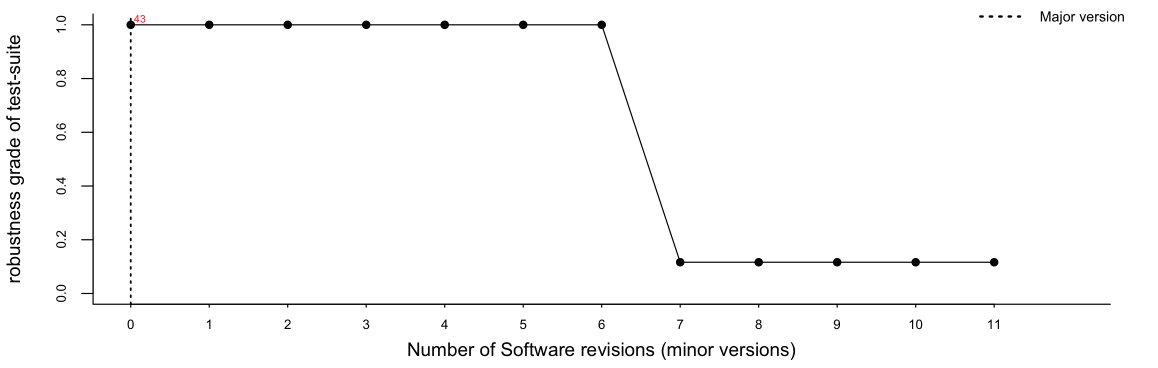
\includegraphics[width=12cm,height=3cm]{./Figures/moodle-rq1}}
\vspace{-2mm}\subfigure[AUT version $V_{1}$]{\label{rob:fireplace}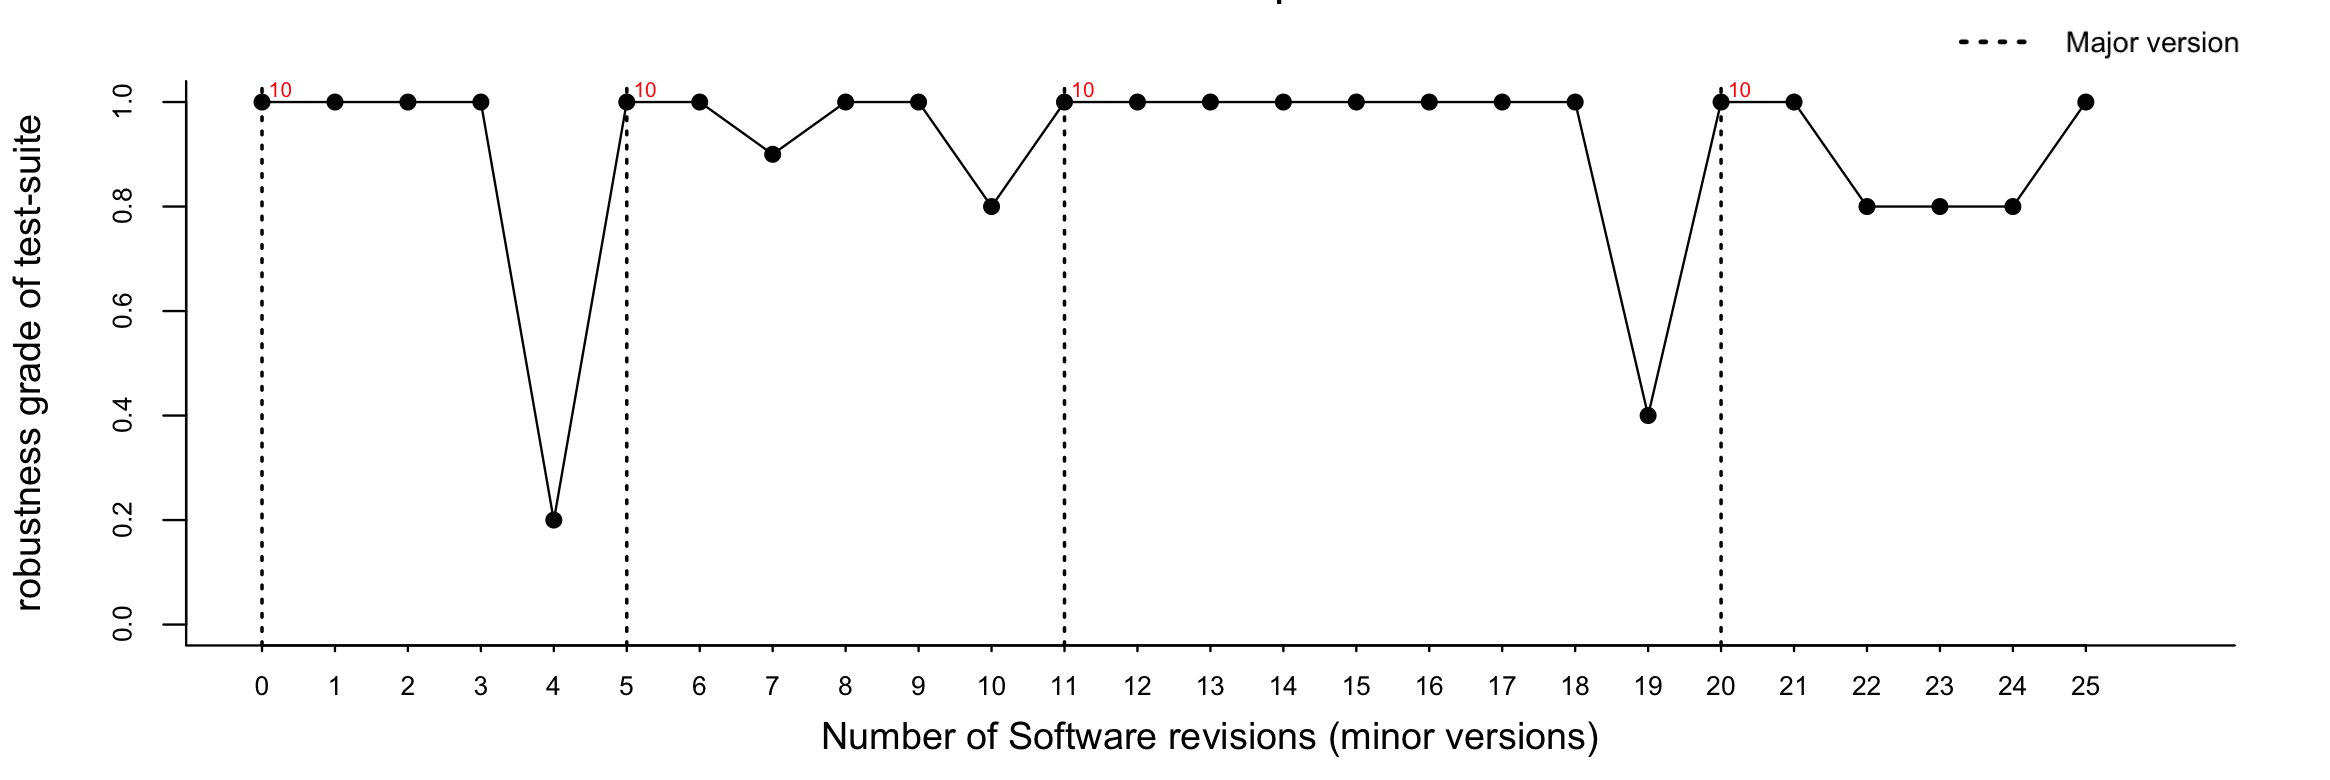
\includegraphics[width=12cm,height=3cm]{./Figures/fireplace-rq1}}
\subfigure[AUT version $V_{0}$]{\label{rob:moodle}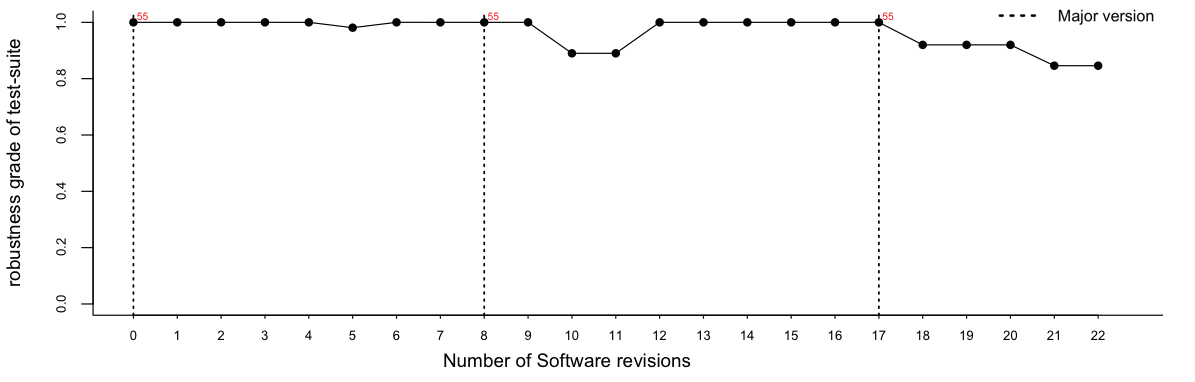
\includegraphics[width=12cm,height=3cm]{./Figures/amo-rq1}}
\vspace{-2mm}\subfigure[AUT version $V_{1}$]{\label{rob:amo}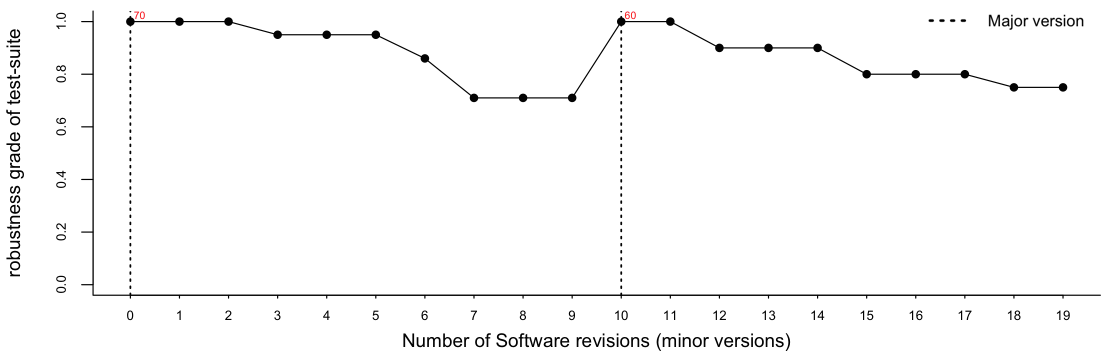
\includegraphics[width=12cm,height=3cm]{./Figures/bedrock-rq1}}
\captionsetup{justification=justified,
singlelinecheck=false}
\vspace{-2mm}\subfigure[AUT version $V_{1}$]{\label{rob:amo}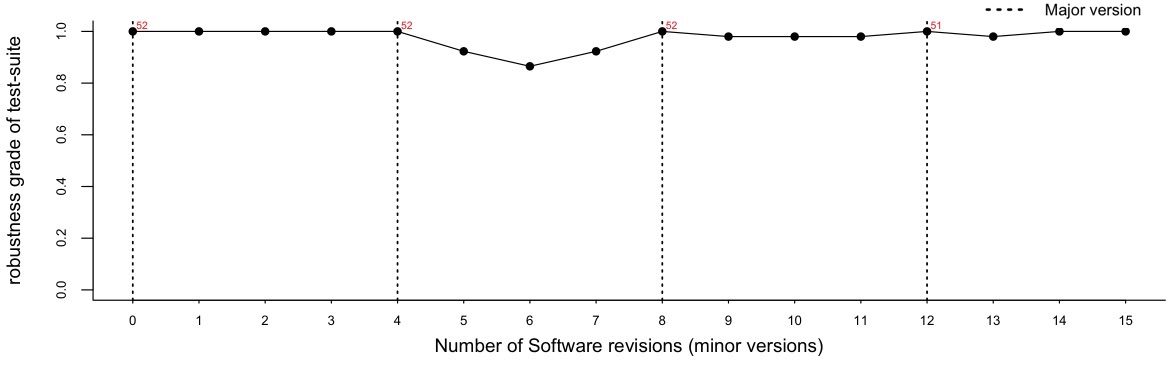
\includegraphics[width=12cm,height=3cm]{./Figures/jenkinsLTS-rq1.jpg}}
\vspace{-2mm}\subfigure[AUT version $V_{1}$]{\label{rob:fireplace}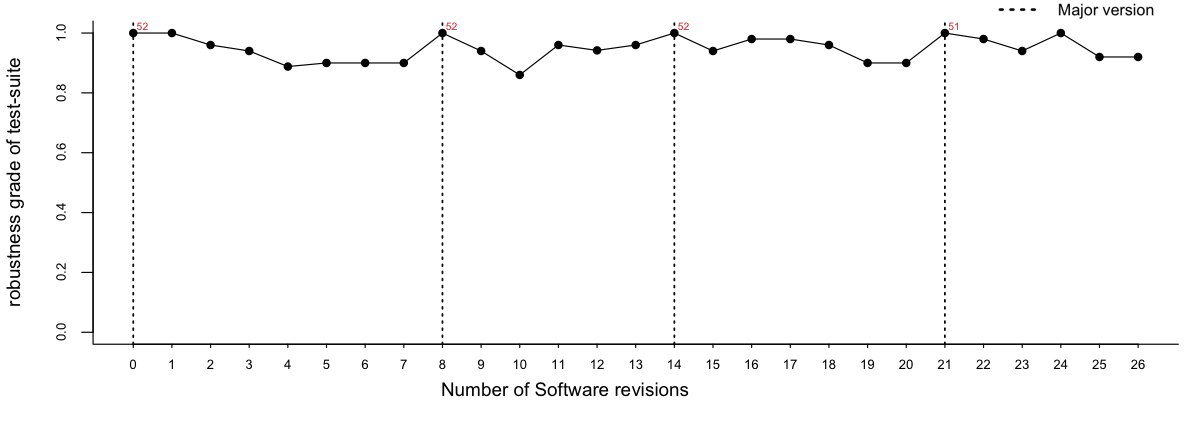
\includegraphics[width=12cm,height=3cm]{./Figures/jenkinsWeekly-rq1.png}}
\caption{Robustness grade $R_{TS_{V_{0}V_{1}}}$ of a test-suit measured across different revisions of AUT. The x-axis represents a software revision, the filled dots (black color) represent }
\label{fig:robustnessplots}
\end{figure} 